\chapter{Positive Kaon Cross Section Measurement}\label{ch:KaonXS}
{\raggedleft ``\emph{Beat-up little seagull, on a marble stair} \par}
{\raggedleft \emph{Tryin' to find the ocean, lookin' everywhere.}"\par}
{\raggedleft -- Nina Simone, 1978 -- \par}% Baltimore,
\vspace{0.5cm}

In this chapter, we show the result of the thin slice method to measure  the ($K^+$-Ar) total hadronic cross section. In Section \ref{ch:KaonXSRaw}, we start by measuring the raw cross section. In Section \ref{ch:KaonXSCorrections}, we apply a statistical subtraction of the background contributions based on simulation and a correction for detection inefficiency. The final results are presented in Section \ref{ch:FinalKaon}.


\section{Raw Cross Section}\label{ch:KaonXSRaw}
We measure the raw ($K^+$-Ar) total hadronic cross section as a function of the kinetic energy in the combined +60A and +100A dataset. 

Similar to the pion case,  the raw cross section is given by the equation \ref{eq:thinTargetXSSolved}
\begin{equation}
 \sigma_{TOT} (E_i)  = \frac{1}{n \delta X}\frac{N^{\text{TOT}}_{\text{Int}}(E_i)}{N^{\text{TOT}}_{\text{Inc}}(E_i)},
\end{equation}

where $N^{\text{TOT}}_{\text{Int}}$  is the measured number of particles interacting at kinetic energy $E_i$, $N^{\text{TOT}}_{\text{Inc}}$ is the  measured  number of particles incident  on an argon slice at  kinetic energy $E_i$,  $n$ is the density of the target centers  and $\delta X$ is the thickness of the argon slice. The density of the target centers and the slab thickness are $n = 0.021\cdot10^{24} \text{ cm}^{-3} $ and  $\delta X=0.47\text{ cm}$, respectively.


As in the case of pions, kaons might decay or interact between WC4 and the TPC front face. Some of the interaction products may be wrongly matched to the WC track, forming the ``secondary" particle's background in the kaon sample. We estimate the effect of the contamination of secondaries through  the DDMC kaon sample.
Figure \ref{fig:InteractingRawK} shows the distribution of  $N^{\text{TOT}}_{\text{Int}}$  as a function of the kinetic energy. The data central points are represented by black dots, the statistical uncertainty is shown in black, while the systematic uncertainty is shown in red. Data is displayed over the $N^{\text{TOT}}_{\text{Int}}$  distribution obtained with a DDMC  sample of kaons shot from WC4.  
The contribution from the simulated kaons which interact hadronically is shown in pink, the contributions from kaon decay is shown in orange and the one from secondaries in red. 
The simulated kaon's and secondaries' contributions are stacked; the sum of their integrals is normalized to the integral of the data.
 
Figure \ref{fig:IncidentRawK} shows the distribution of  $N^{\text{TOT}}_{\text{Inc}}$. Data is displayed over the MC. For the  $N^{\text{TOT}}_{\text{Inc}}$ distribution we do not make a distinction between kaons that decay or interact hadronically because any kaon independently from its final interaction contributes to the flux of incident particles at given kinetic energy.
The same normalization procedure is used for both the interacting and incident histograms. 


Figure \ref{fig:XSRawK} shows the raw cross section, statistical uncertainty in black and systematic uncertainty in red. The raw data cross section is overlaid to the reconstructed cross section for the MC mixed sample, displayed in azure.  We calculate the statistical uncertainty for the interacting, incident and cross section distributions in a similar fashion to the pion case as described in Section \ref{ch:StatUncertaintyXSRaw}. 

As in the pion case, the only systematic effect considered in the measurement of the raw cross section results from the propagation of the uncertainty associate with the measurement of the kinetic energy at each argon slab. For kaons, the uncertainty on the kinetic energy of a candidate at the j$^{th}$ slab of argon  is given by

\begin{eqnarray}
\delta KE_{j} &=& \sqrt{\delta p_{Beam}^2 + \delta E_{Loss}^2 +  \delta  E_{\text{dep FF-j}}^2}\\
&=& \sqrt{(2\% \text{ }p_{Beam})^2 +  (7 \text{ [MeV]})^2 +  (j-1)^2 (\sim0.18\text{ [MeV]})^2}.
\end{eqnarray}

We propagate this uncertainty  by varying the energy measurement $KE_{j}$ at each argon slab. We measure $N^{\text{TOT}}_{\text{Inc}}$,  $N^{\text{TOT}}_{\text{Int}}$ and the cross section  in three cases: first assigning the measured $KE_{j}$ at each kinetic energy sampling, then assigning $KE_{j} + \delta KE_{j}$, and finally assigning $KE_{j} - \delta KE_{j}$. The difference between the values obtained using the $KE_{j}$ sampling and the maximum and minimum values in each kinetic energy bin determines the systematic uncertainty.

\begin{figure}[]
\centering
\begin{minipage}[t]{0.45\textwidth}
\centering
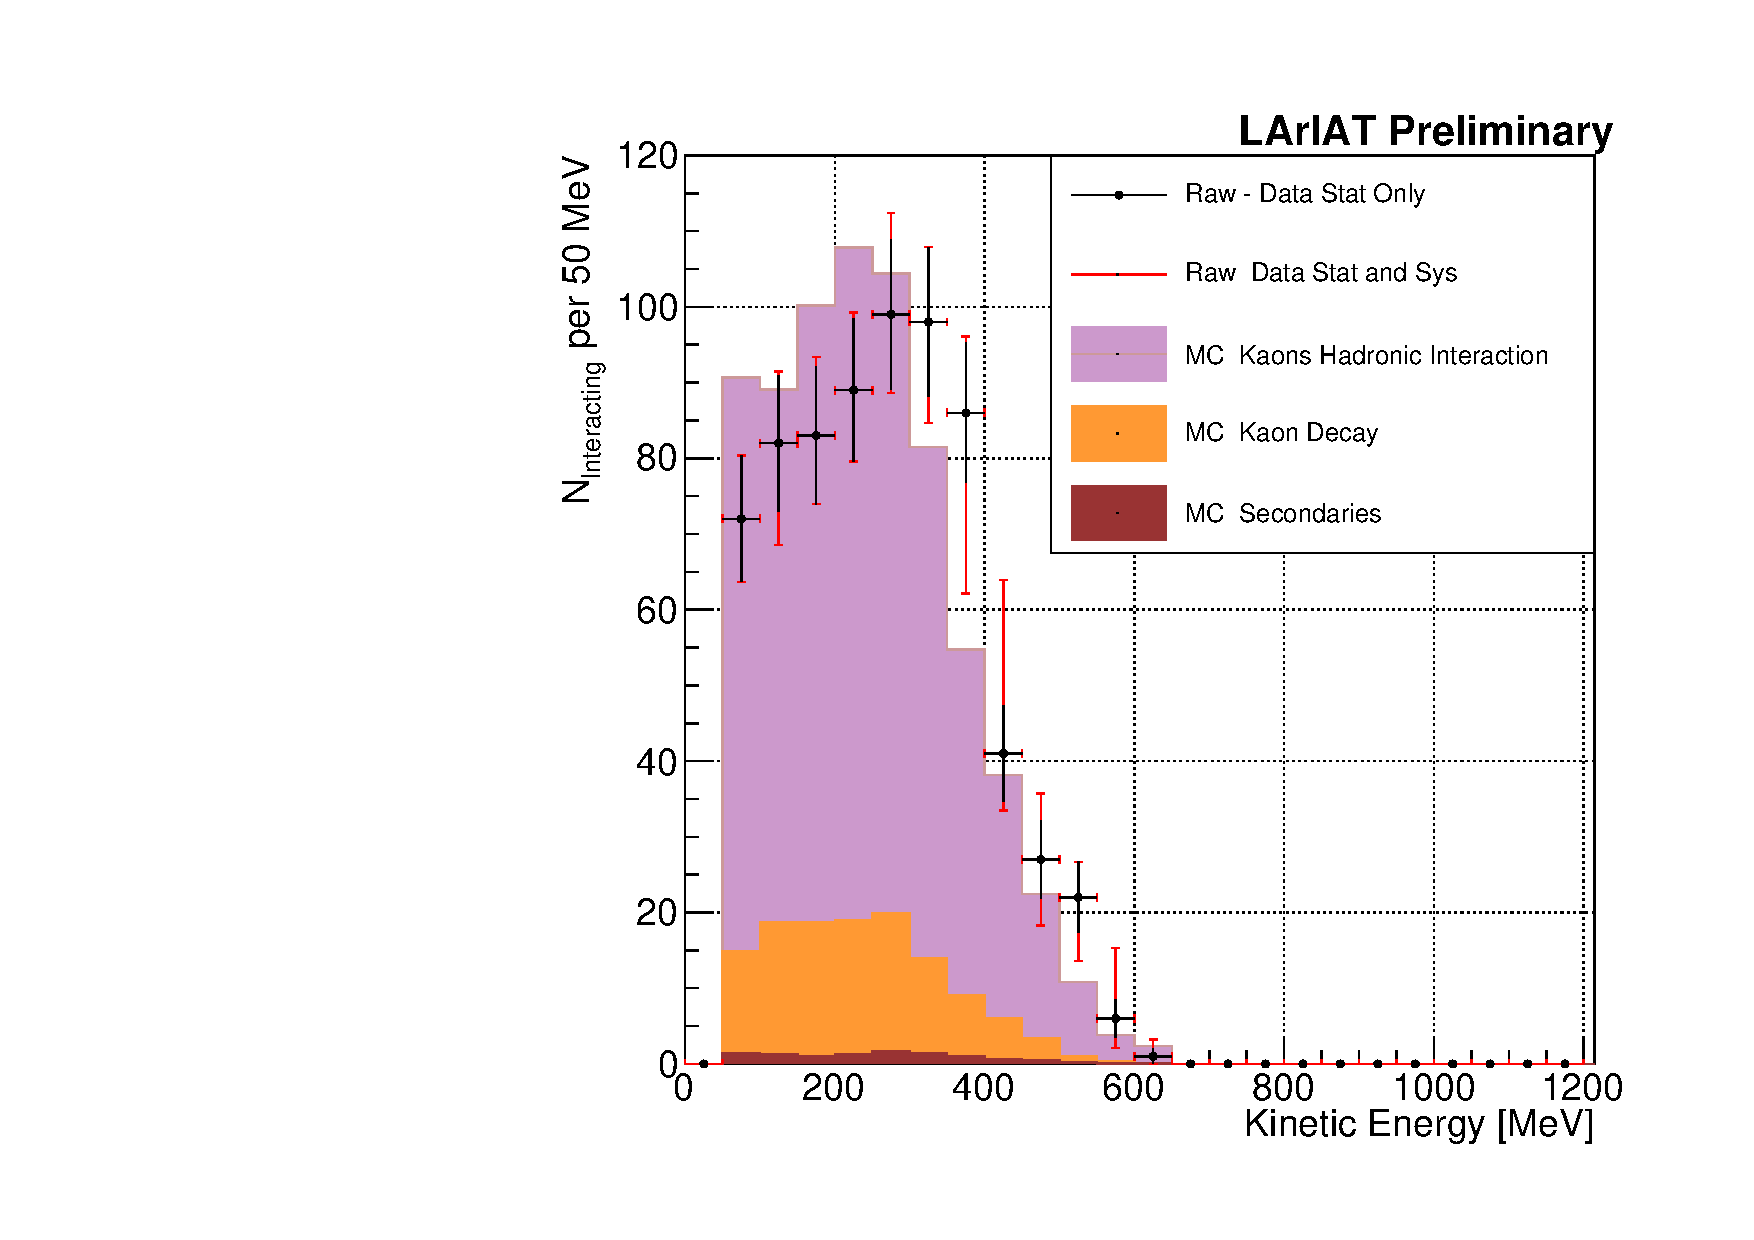
\includegraphics[width=\textwidth]{Chapter-7/Images/Plots_MCData_Int_StatSystK_WithDK.pdf}
\caption{Raw number of interacting kaon candidates as a function of the reconstructed kinetic energy. The statistical uncertainties are shown in black, the systematic uncertainties in red.}
\label{fig:InteractingRawK}
\end{minipage}\hfill
\begin{minipage}[t]{0.45\textwidth}
\centering
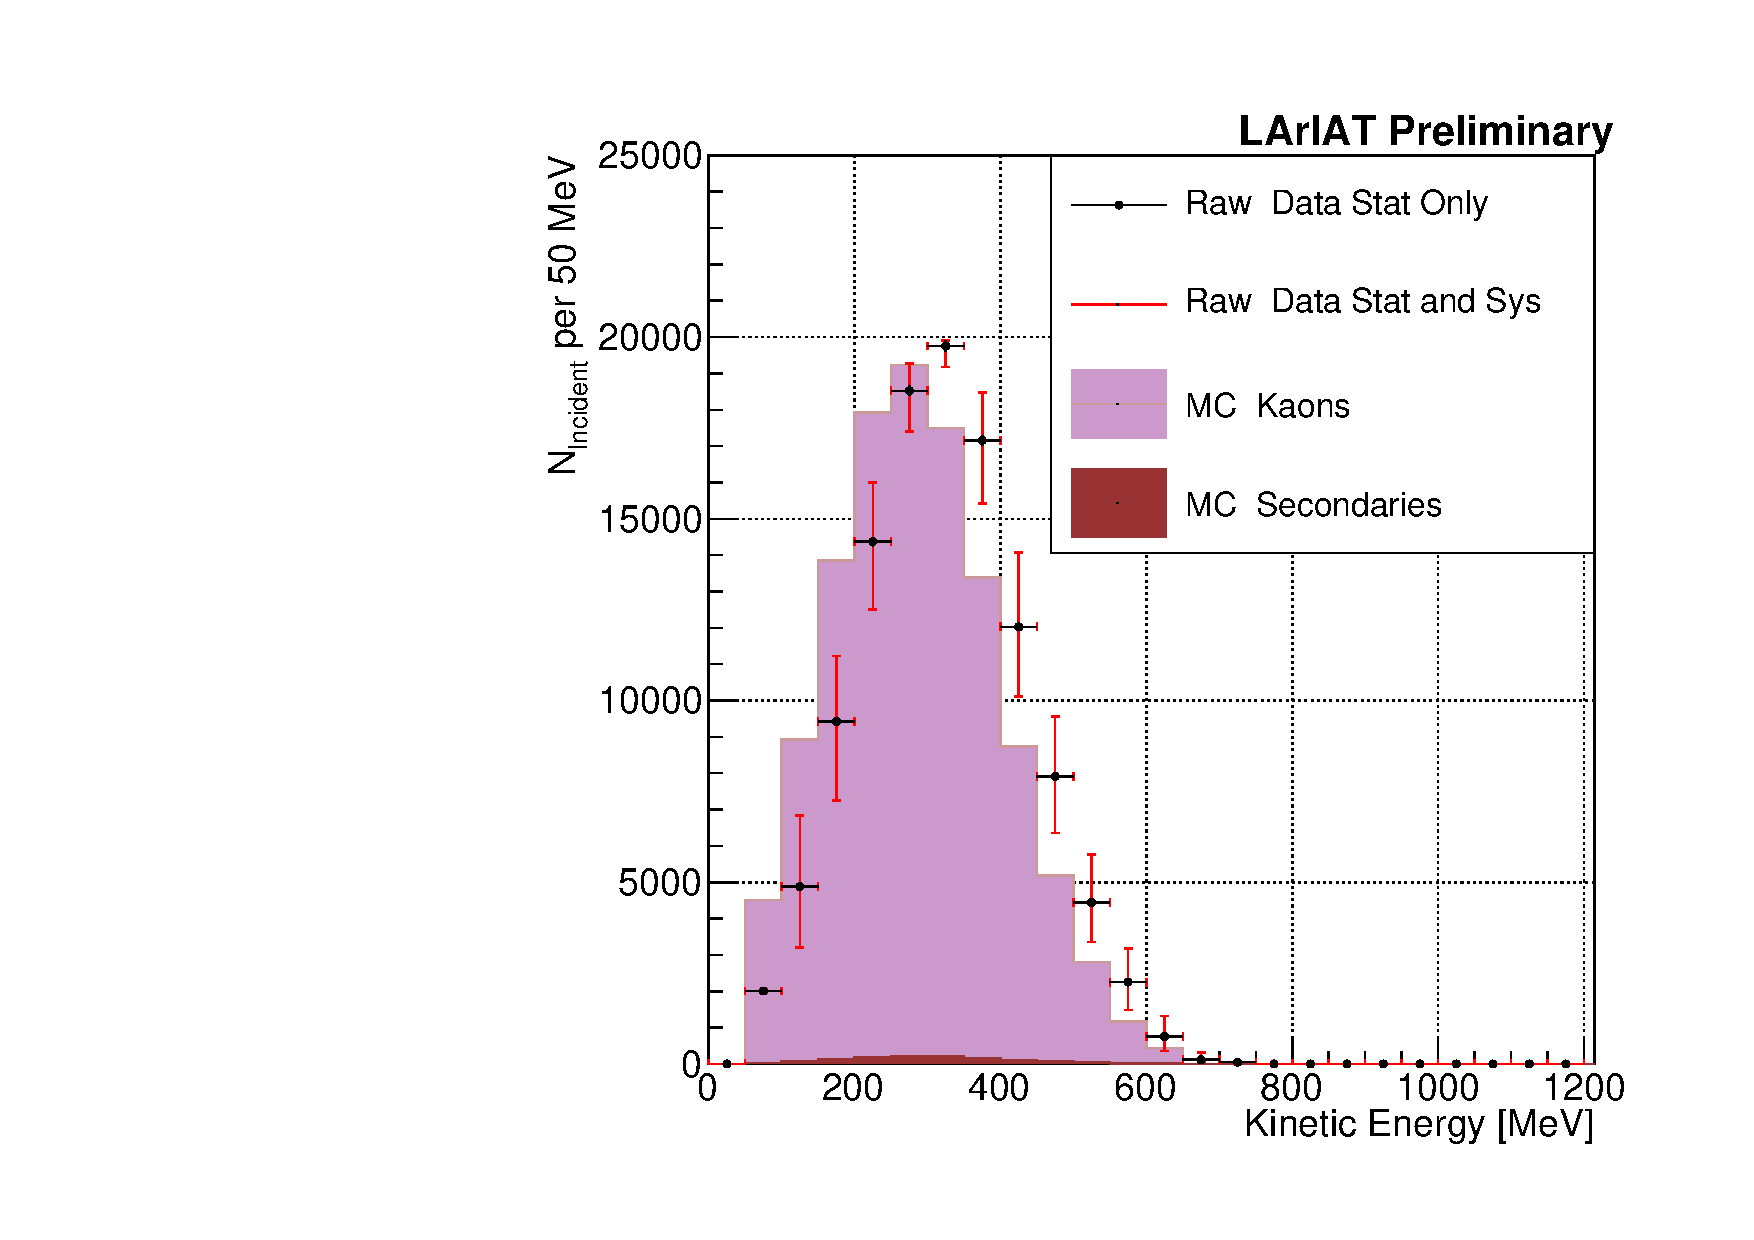
\includegraphics[width=\textwidth]{Chapter-7/Images/Plots_MCData_Inc_StatSystK_WithDK.pdf}
\caption{Raw number of incident kaon candidates as a function of the reconstructed kinetic energy. The statistical uncertainty is shown in black, the systematic uncertainties in red.}
\label{fig:IncidentRawK}
\end{minipage}
\end{figure}



\begin{figure}
\centering  
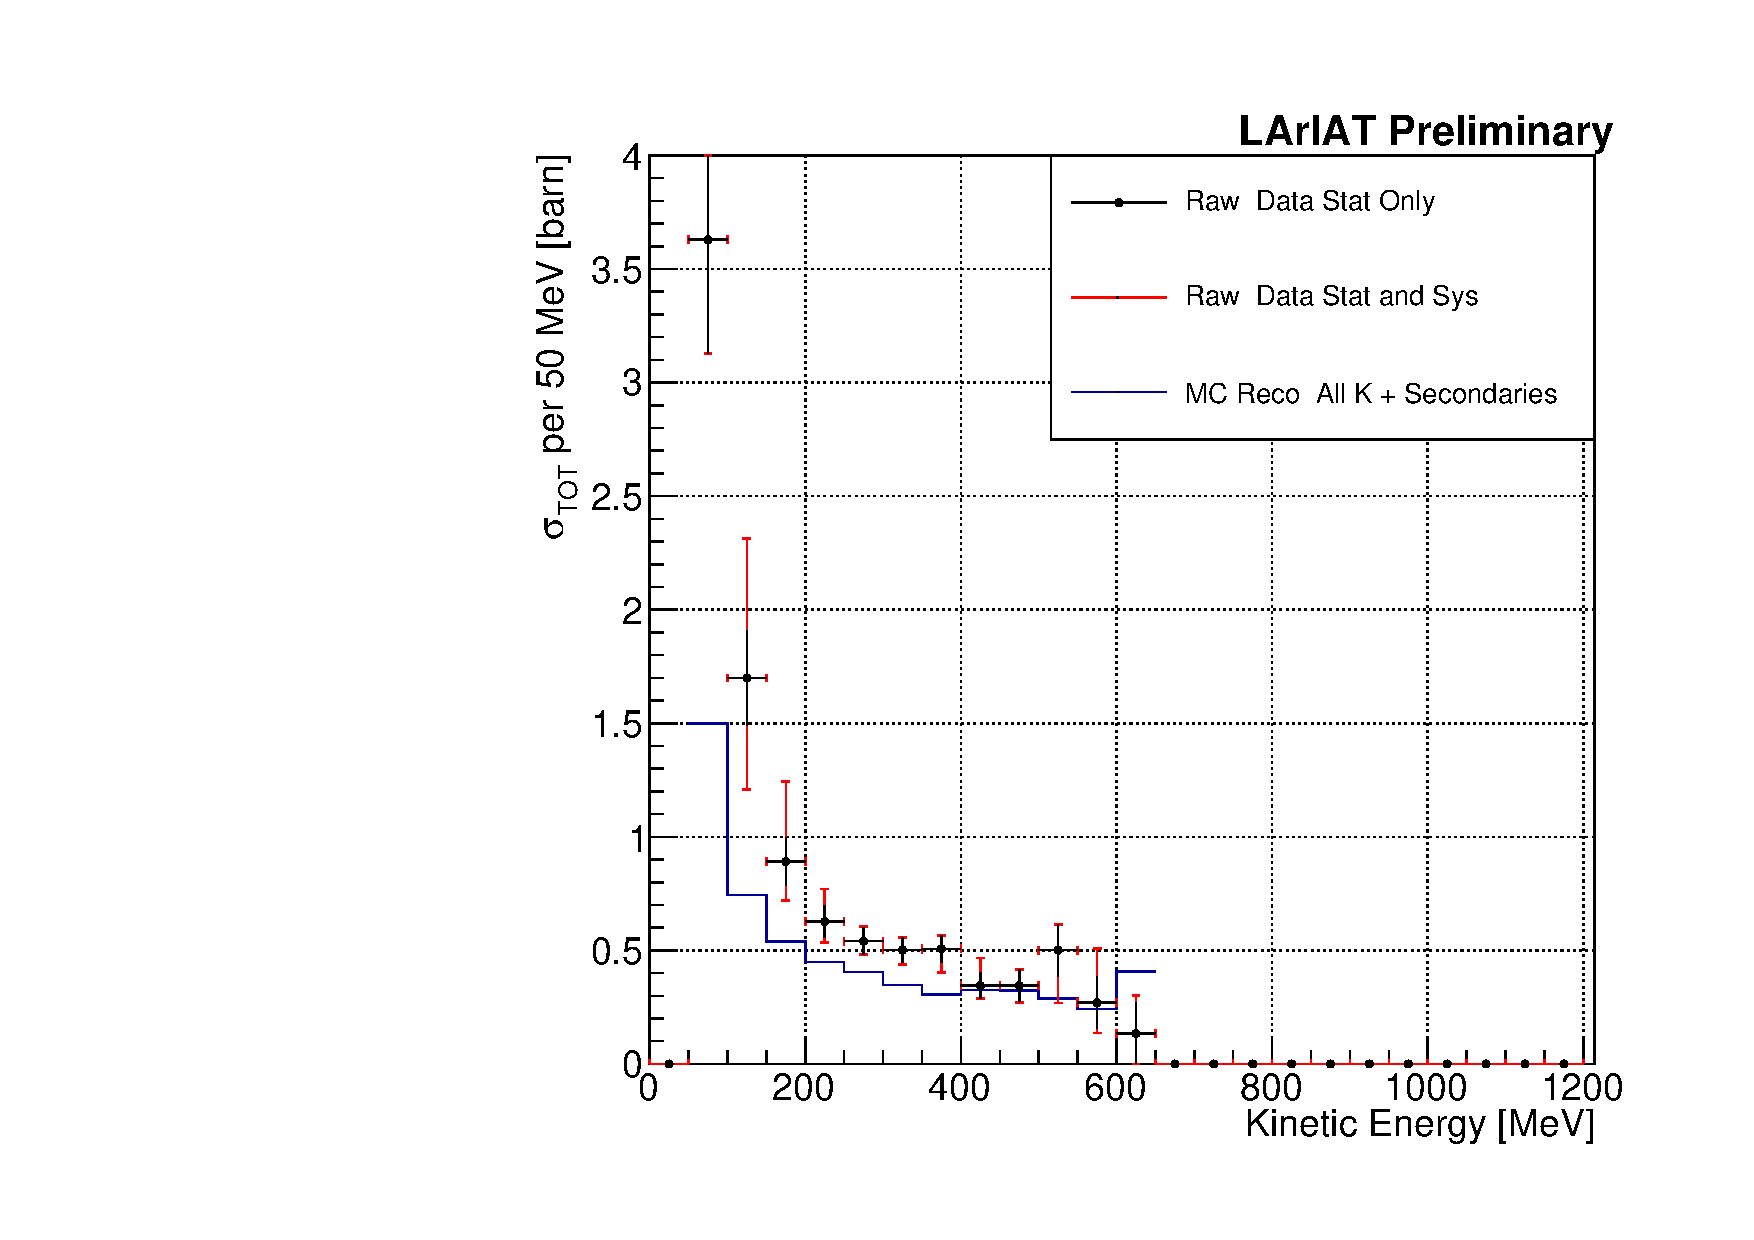
\includegraphics[width=0.48\textwidth]{Chapter-7/Images/Plots_MCData_XS_StatSystK_WithDK.pdf}
\caption{Raw ($K^+$-Ar) total hadronic cross section. The statistical uncertainty is shown in black, the systematic uncertainties in red. The raw cross section obtained with a MC sample of kaons is shown in azure. For the MC cross section,  we include the contributions from secondaries. }
\label{fig:XSRawK}
\end{figure}


\section{Corrections to the Raw Cross Section}\label{ch:KaonXSCorrections}
As described in section \ref{ch:MCCorrections}, we need to apply a background correction and an efficiency correction in order to derive the true Kaon cross section from the raw cross section.  The true cross section is given in equation \ref{eq:C}, 

\begin{equation}
   \sigma^{K^+}_{TOT}(E_{i})  = \frac{1}{n \delta X}\frac{ \epsilon^{\text{Inc}}(E_i)  \hspace{0.2cm} C^{K MC}_{\text{Int}} (E_{i}) \hspace{0.2cm} N^{\text{TOT}}_{\text{Int}} (E_{i}) }{   \epsilon^{\text{Int}}(E_i) \hspace{0.2cm} C^{K MC}_{\text{Inc}} (E_{i}) \hspace{0.2cm}  N^{\text{TOT}}_{\text{Inc}} (E_{i})}.
 \tag{\ref{eq:C}}
\end{equation}

Currently, the only background considered for the kaon hadronic cross section comes from the presence of secondaries. A further development of the analysis will need to account for the presence of a small proton contamination. Figure \ref{fig:CorrectionsBeamK} shows the relative kaon content for the interacting and incident histograms.
\begin{figure}[p]
\centering
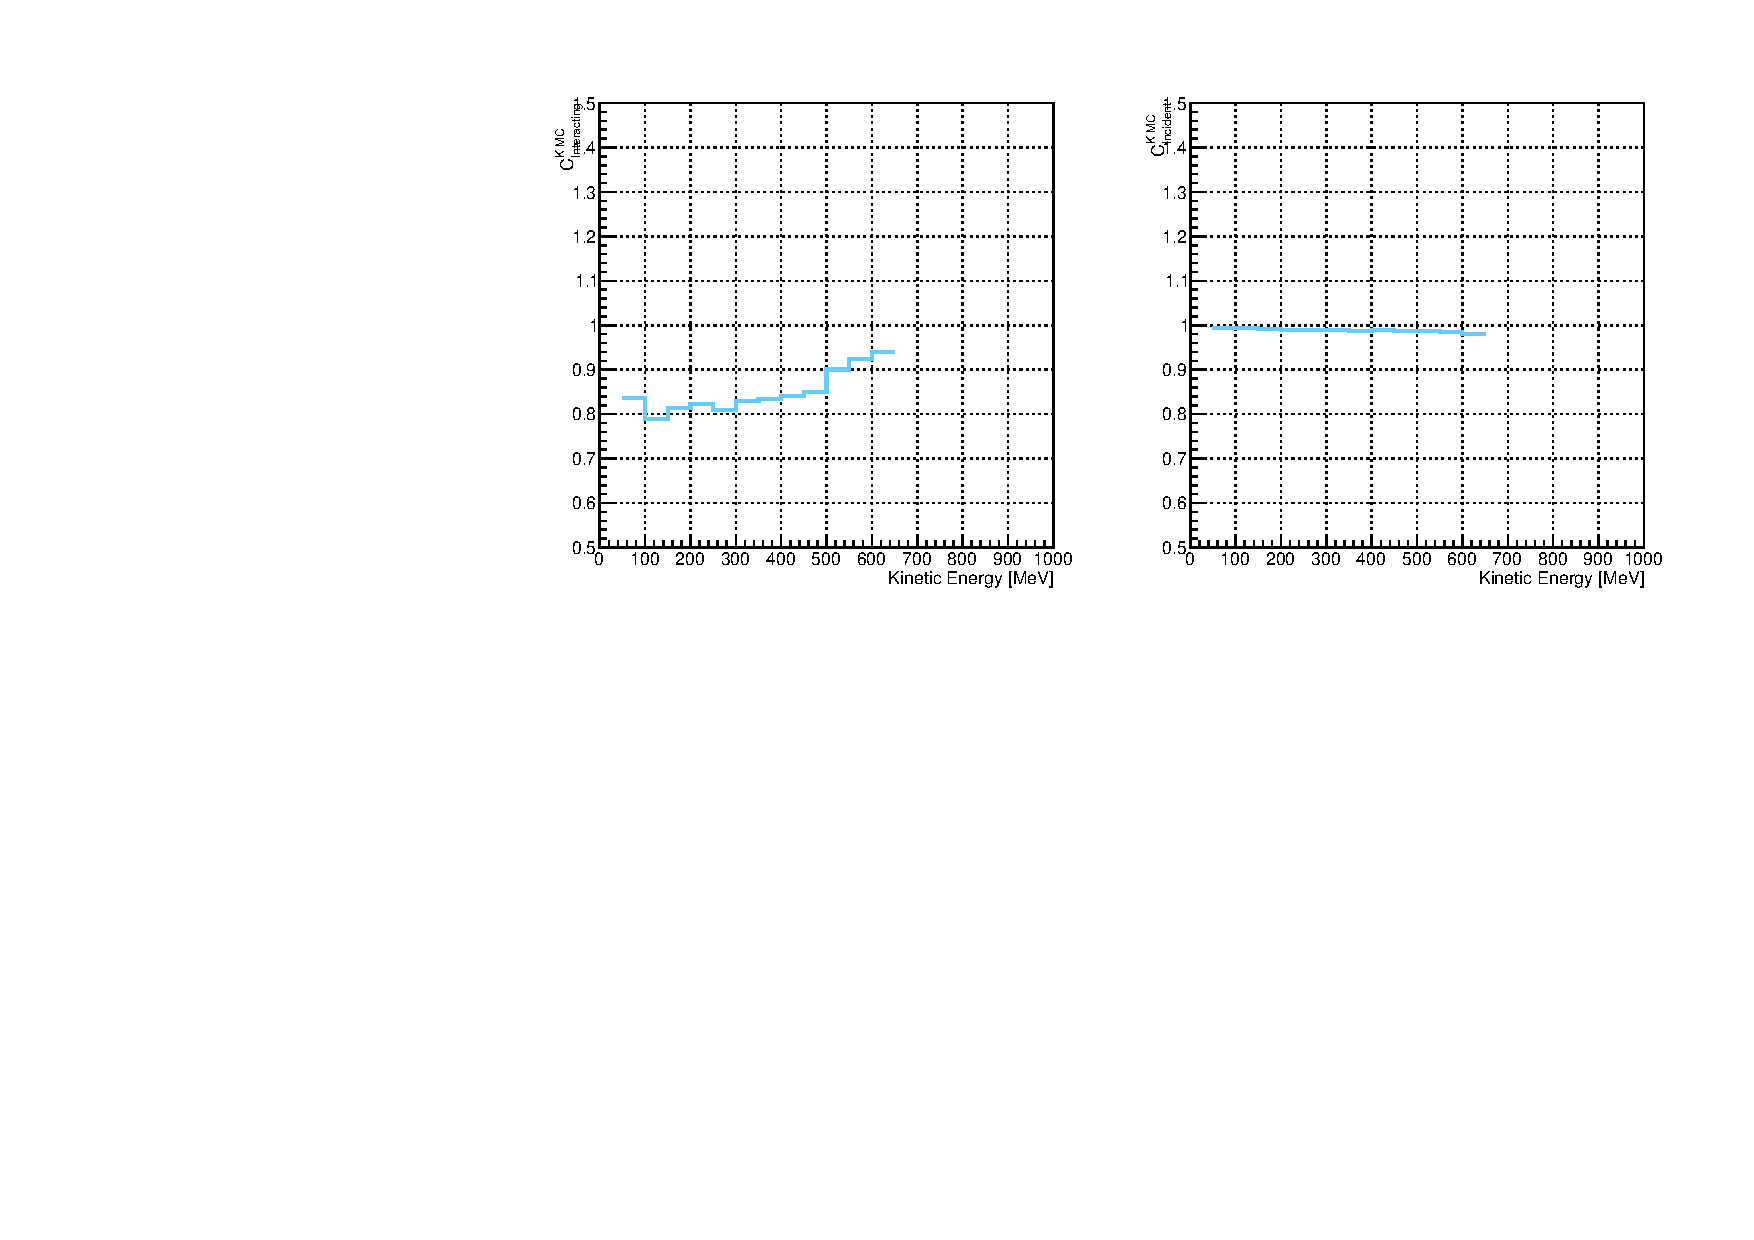
\includegraphics[width=\textwidth]{Chapter-7/Images/KaonBkgSub_WithDK.pdf}
\caption{\emph{Left:} MC estimated relative kaon content for kaons interacting hadronically as function of kinetic energy. \emph{Right:}  MC estimated relative kaon content  for incident histogram a function of kinetic energy.}
\label{fig:CorrectionsBeamK}
\end{figure}


As described in \ref{ch:EFFXS} for the pion case, we derive the correction on a set of pure kaon MC, calculating its value bin by bin as the ratio between the true bin content and the correspondent reconstructed bin content. The correction is then applied to the relevant bin in data. 
The efficiency correction is evaluated separately for the interacting and incident histograms, namely $\epsilon^{\text{int}}_i$ and  $\epsilon^{\text{inc}}_i$, and propagated to the cross section as shown in  equation \ref{eq:C}. 


In section \ref{sec:angleRes}, we estimated the angular resolution for data and MC to be $\bar\alpha_{Data} = (4.3 \pm 3.7) \text{ deg}$  and  $\bar\alpha_{MC} = (4.4 \pm 3.6) \text{ deg}$, respectively.  Most interaction angles smaller than the angular resolution will thus be indistinguishable  for the reconstruction. Thus, we claim we are able to  measure the cross section for interaction angles greater than 4.5 deg. Geant4 simulates interactions at all angles: in order to calculate the efficiency correction,  we select events which have an interaction angle greater than a $\alpha_{res}$ to construct the true interacting and incident histograms (the denominator of the efficiency correction). The systematics on the efficiency correction is estimated by varying the value of $\alpha_{res}$ between 0 deg and 4.5 deg and propagating the uncertainty on the cross section. 

Figure \ref{fig:EffCorrK} shows $\epsilon^{\text{Int}}(E_{i})$ in the left side and $ \epsilon^{\text{Inc}}(E_i)$ on the right as a function of the kinetic energy for the kaon sample and their systematic uncertainty. 


\begin{figure}
\centering
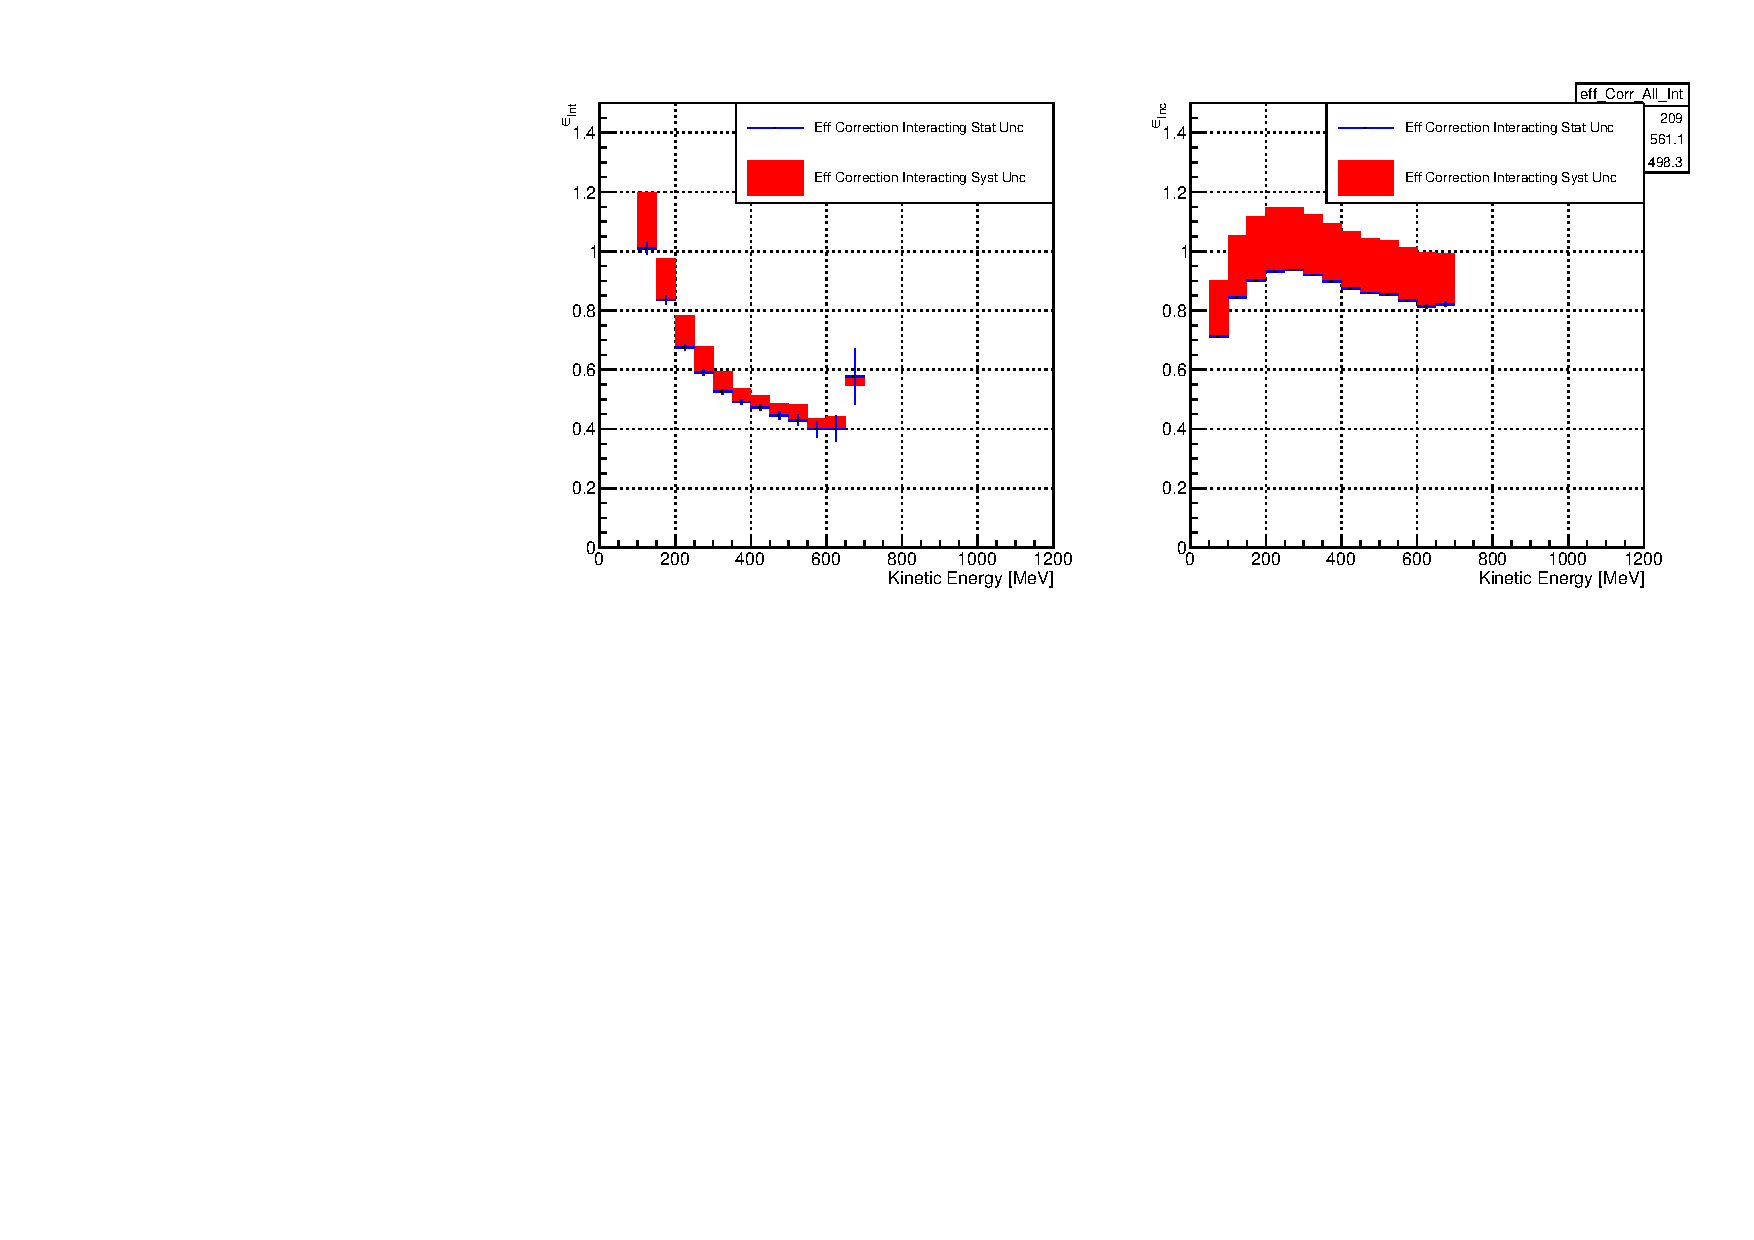
\includegraphics[width=\textwidth]{Chapter-7/Images/EffCorrK.pdf}
\caption{\emph{Left:} Efficiency correction on the interacting histogram, statistical uncertainty in blue, systematic uncertainty in red. \emph{Right:}  Efficiency correction on the incident histogram, statistical uncertainty in blue, systematic uncertainty in red.}
\label{fig:EffCorrK}
\end{figure}



\section{Results}\label{ch:FinalKaon}
Figure \ref{fig:FinalXSKaon} show the measurement of the ($K^+$-Ar) total hadronic cross section for  scattering angles greater than 5$^\circ$, as the result of the background subtraction and efficiency correction to the raw cross section. The plot shows the measurement obtained on the full dataset, statistical uncertainty in black and systematic uncertainty in red. The Geant4 prediction for the total hadronic cross section for angle scattering greater than 5$^\circ$ is displayed in green.

The systematic uncertainty on the cross section is the sum in quadrature of the statistical uncertainty, the systematic uncertainty related to the kinetic energy measurement and the systematic uncertainty related to the efficiency correction.

\begin{figure}[htb]
\centering
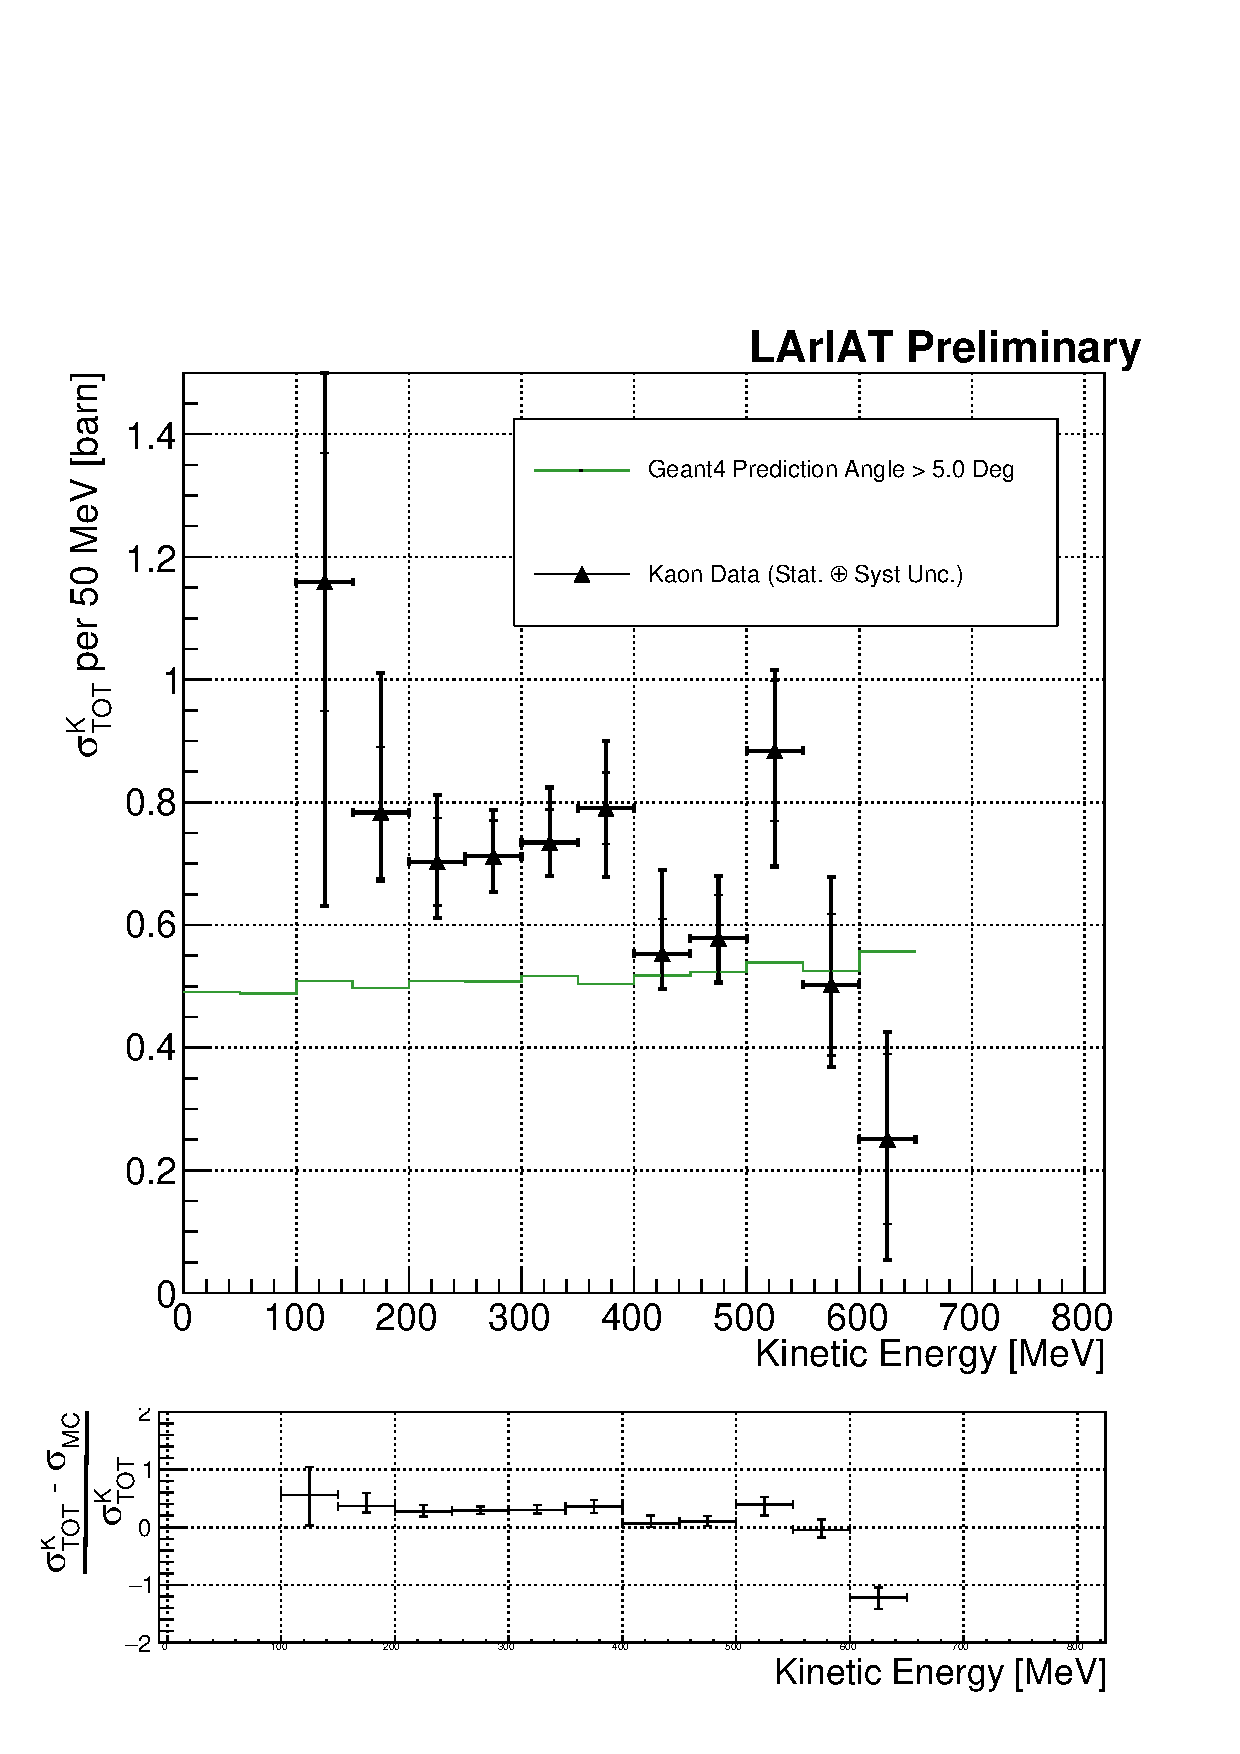
\includegraphics[width=0.48\textwidth]{Chapter-7/Images/TheMoneyPlotK.pdf}
\caption{ ($K^+$-Ar) total hadronic cross section for  scattering angles greater than 5$^\circ$ measured in the 60A sample, statistical uncertainty in black and systematic uncertainty in red. The Geant4 prediction for the total hadronic cross section for angle scattering greater than 5$^\circ$ is displayed in green. } 
\label{fig:FinalXSKaon}
\end{figure}


%%%%%%%%%%%%%%%%%%%%%%%%%%%%%%%%%%%%%%%%%%%%%%%%%%%%%%%%%%%%%%%%%%
\begin{comment}





\clearpage
\section{Results}\label{ch:FinalKaon}


\end{comment}

